\chapter{UPPAAL model}\label{ch:uppaalmodel}
In this chapter, we describe, how we model modular factory configurations. In addition, we will explain, how we may rate a configuration by producing its fastest schedule through simulation. We want to be able to model and simulate configurations, so that we may compare the ratings of many different configurations. This would not be practical, if we had to set up each configuration physically.

To model modular factories and simulate individual configurations, we use the UPPAAL model-checker\cite{Larsen97uppaalin}. This is an integrated development environment used for modelling, simulating and verifying real-time systems. It allows us to model our system using timed automata in a combined graphical and programmatic manner. Once we have designed our model, we may use it to instantiate a configuration and a set of items. UPPAAL can then simulate the production of these items on the given configuration. In addition, the model-checker included in UPPAAL, allows us to query different properties about the setup. To us, the most interesting property is one of reachability; \textit{Is it possible to reach a state, where all items in an order have been produced?} If this is the case, then UPPAAL may produce a fastest timed trace of transitions needed to reach this state. This sequence of system states evaluates to the fastest schedule for the given configration. Looking at the global clock of the final state in the trace gives us the time taken to execute the trace, and thus our configuration rating.

UPPAAL has been used to model many different real-life systems, such as a lacquer\cite{so54514} and an industrial printer\cite{Igna2008}. From this research we take inspiration for our model. In these examples however, UPPAAL is used to model systems with only a single configuration. Our work differs in that we attempt to model a system of which there are many possible configurations, which need to be compared. Therefore we focus on keeping the module flexible and avoiding hard-coded values. Thus, many different configurations and items may be instantiated.

When modeling the real world, we need to take care to pick an appropriate abstraction level. Too high, and the model will not fit well with the real world. Too low and the model becomes very complex. The more complex a model is, the more likely it is that the search space will be large. This severely increases the runtime, when searching for a best schedule. Therefore, we naturally aim to hit a sweet spot between abstraction and complexity.

In this chapter we will explain how we modeled configurations and items in UPPAAL, so that we may simulate production. This will be a look at both the technical implementation, but also a discussion on when we have abstracted from the real world, and when we have not. We will also extend the design decision made in \cref{sec:runningexample}. 

\section{Recipe}\label{sec:recipe}
In this section, we will describe how we modelled items that are produced by a modular factory. Looking into earlier projects developed using UPPAAL, an item being produced is often implemented as a sequence of actions, which must be taken in order to complete the item. Therefore items are often refered to as recipes. We will do the same from this point on. 

There are of course different ways of implementing a recipe. The most simple variant is a list of actions, which must be performed linearly. However, we find it more flexible to implement a recipe as a dependency graph. This is because we often do not care for the precise sequence of actions, just that some actions are performed before others. This is easily described using a dependency graph as seen in \cref{fig:dependency-graph}. This recipe describes that it needs to be hammered and screwed before it is packaged, yet it cares not in which order the hammering and scewing takes place. 

We know that in some real life systems, a single item may be created through the aggregation of parts, which are individually produced. To escape this complexity, we only consider items, whose production is never distributed. That is the production of an item starts at one single point and ends at another point never splitting up. As we represent recipes as dependency graphs, it also means that the same work can not be applied on a recipe several times, as this would produce cycles in graph. 

\begin{figure}[h]
\centering
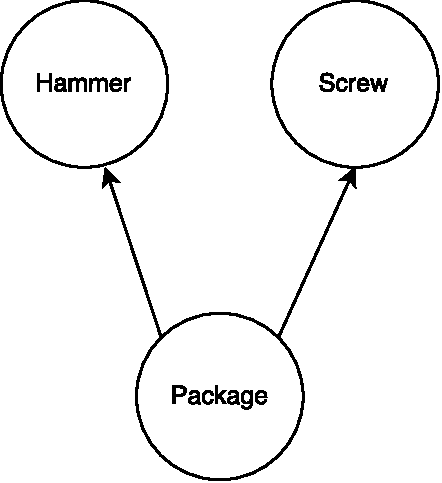
\includegraphics[width=0.3\textwidth]{dependencygraph.pdf}
\caption{Dependency graph describing order of actions}
\label{fig:dependency-graph}
\end{figure}

In \cref{fig:recipe} we present the recipe template. This template may be instantiated with parameters, to produce an instance functioning according to a specific dependency graph. In our implementation, each node of the underlying graph knows the type of work it represents, how many nodes it depends on, which nodes depend on it and how many nodes depend on it. In addition to the functional dependency graph, a recipe also has a unique id, as well as the id for the module, on which it should start processing. 

When a recipe begins processing, it is placed onto its start module, and we find the ids of nodes, which do not depend on any other node. The ids of these are placed into the local \emph{current\_nodes} array, and represent what actions can be performed on the recipe. After this, the recipe is moved along the factory. Each time it meets a module, where it wishes to have an action performed, it will handshake on its own private channel with the module. Afterwards it will synchronize with the module again on one of the allowed \emph{work} channels. As the \emph{handshaking} location is commited the handshake acts as a mutex, ensuring that no other recipe can suddenly be worked by the module. A work channel can be synchronized on, if one of the nodes in the \emph{current\_nodes} array, represent the work type corresponding to that work channel. Once work has been accomplished, the worked node is removed. If this frees up any unworked node in the graph, its id is added to the \emph{current\_nodes} array. When the array is empty, it means that there is no work left to do, and the local \emph{done} boolean is set to \emph{True}. From this point on a recipe can not be worked on any further.


\begin{figure}[h]
\centering
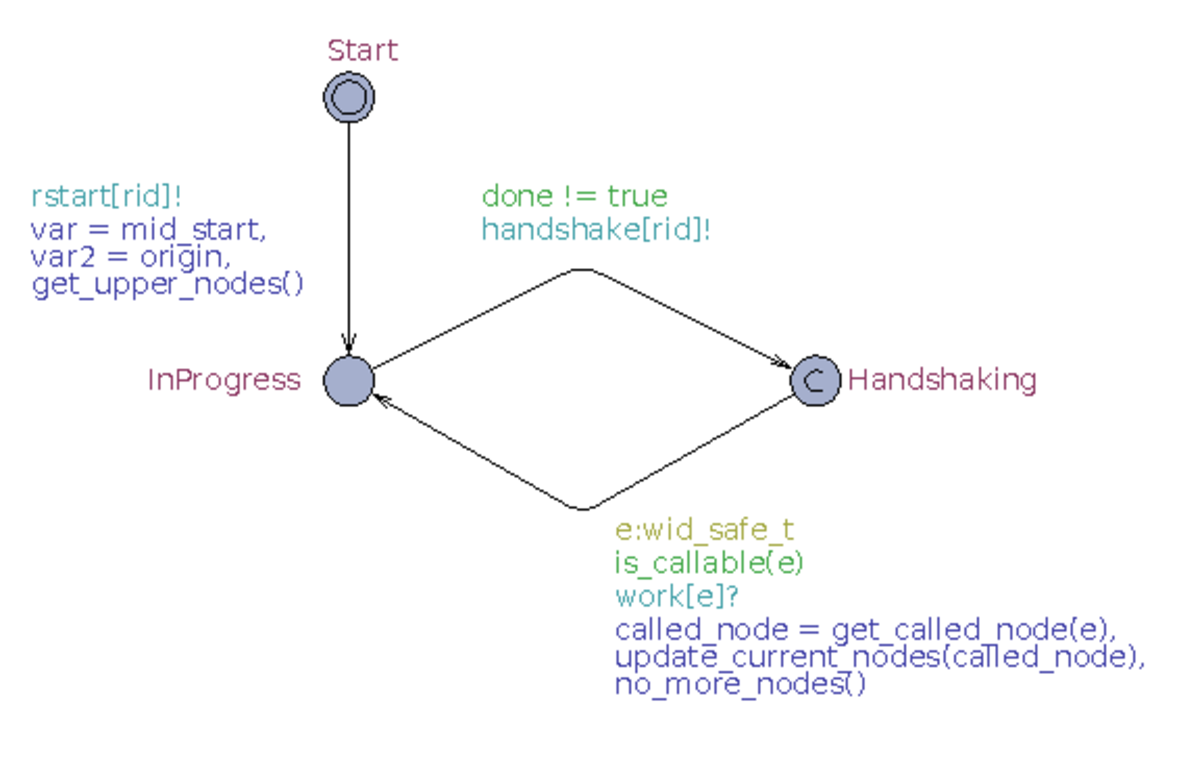
\includegraphics[width=\textwidth]{recipe.pdf}
\caption{Recipe template}
\label{fig:recipe}
\end{figure}

We feel that our \emph{Recipe} template is a rather efficient implementation. However as each recipe instance represents a single item, we quickly get a large state space, if several recipies from the beginning are fighting to get onto the factory line. Therefore we implement a queuing system for recipies through the \emph{RecipeQueue} template as seen in \cref{fig:recipequeue}. This is instantiated with an array of recipe id's indicating the order in which we wish the recipes produced. Once instantiated, the queue may be popped from the front, and the recipe may begin processing. This reduces the state space, as recipes are to begin in a specified order. We will not get into how to produce an efficient ordering of recipes here, as it will be brought up in \cref{ch:configuration}.

\begin{figure}[h]
\centering
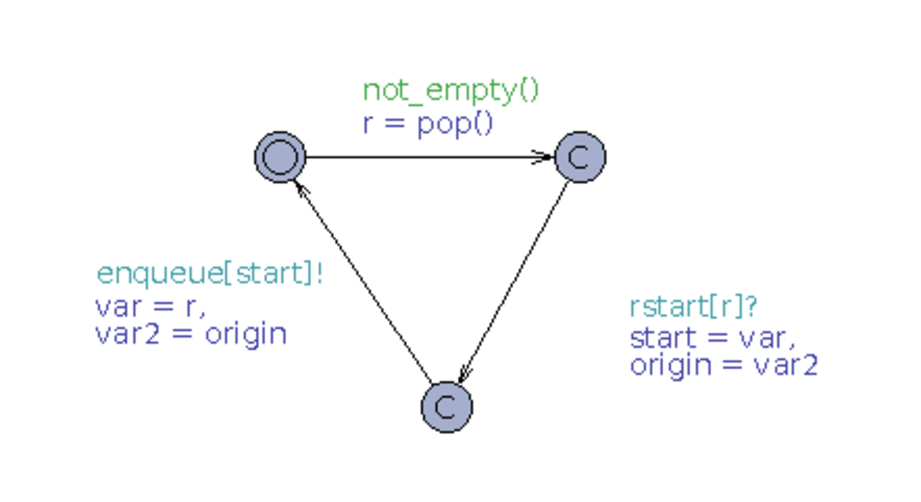
\includegraphics[width=\textwidth]{recipequeue.pdf}
\caption{RecipeQueue template}
\label{fig:recipequeue}
\end{figure}
\section{Module}\label{subs:module}
As a configuration is made up of individual modules, it seems natural to model it as a set of synchronizing module processes. In this section we will first show off the initial design of the \textit{Module} template. Then discuss, how we got more concrete with the final version. 

\subsection{Early Module Template}
In our early design work, we tried to implement most everything brought up in \cref{sec:runningexample}. A module has an identifying name, and it may only work on one item at a time. It also takes a certain amount of time to perform  work and to transport an item across it. However, we start by allowing modules to only perform one type of work. There are also no physical restrictions, on which modules may be connected, other than the fact that a module may not be connected to more than four other modules. These basic ideas turned into our first version of the \textit{Module} template, which can be seen in \cref{fig:earlymodule}.


\begin{figure}[H]
\centering
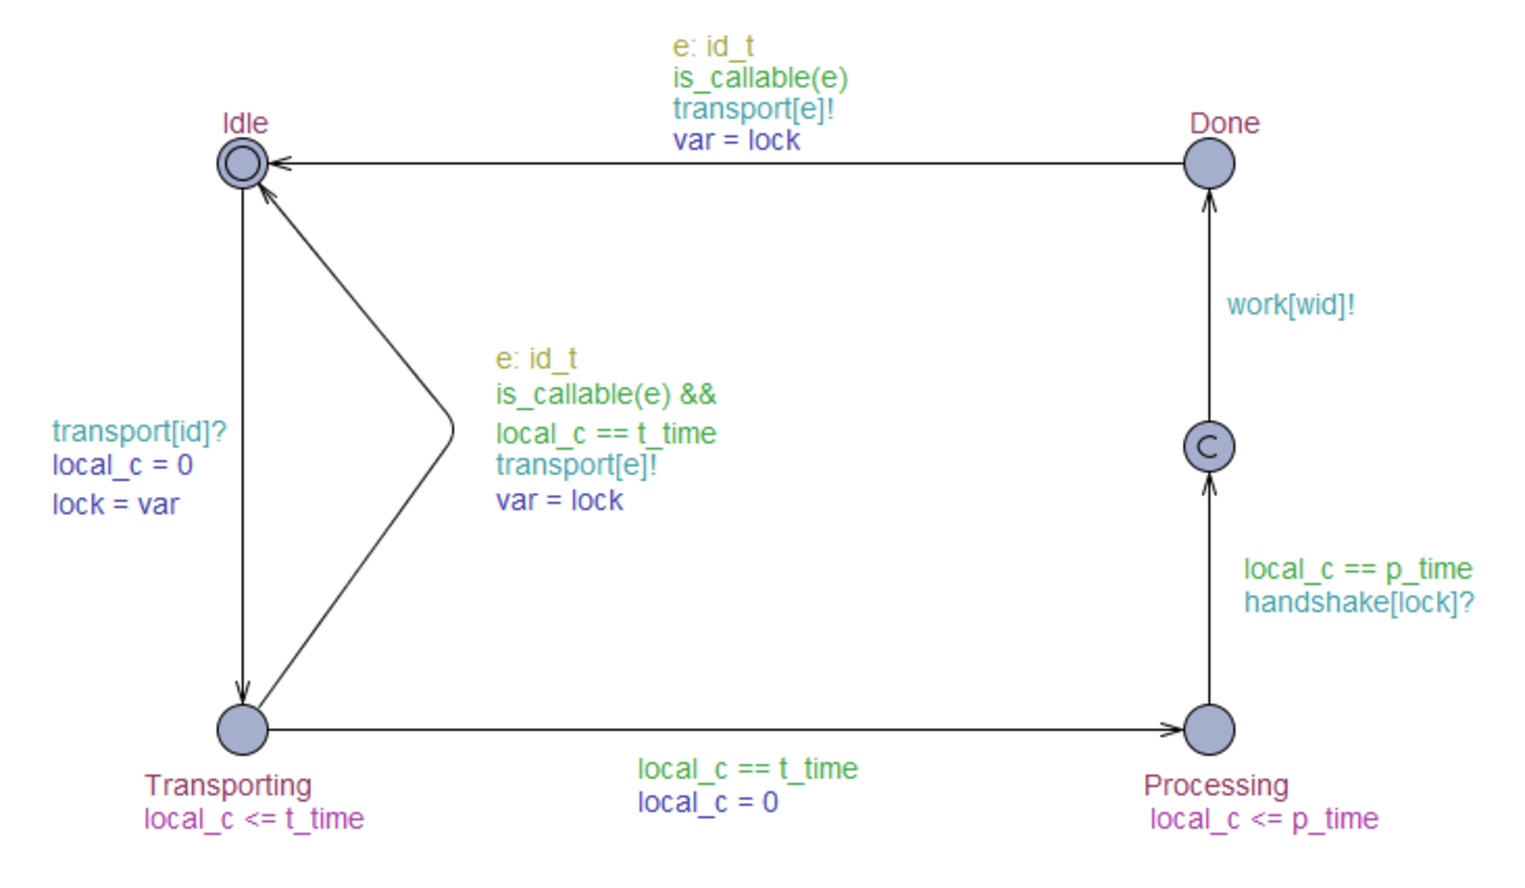
\includegraphics[width=\textwidth]{earlymodule.pdf}
\caption{Early version of the \textit{Module} template}
\label{fig:earlymodule}
\end{figure}

A module starts in the \emph{Idle} location and resides there, when not processing an item. It leaves this location, when one of its up to four neighbouring modules passes on an item by synchronizing on the \emph{transport} channel identified by the modules's id. Once an item has been received, the module waits in the \emph{transporting} location for \emph{t\_time}. This simulates the time taken to transport the item across the module. Once the time has passed we may send the item to a neighbouring module. The local guarding function \emph{is\_callable} makes sure, we only send to neighbours. This set-up allows us to implement modules, which are only used for transporting item.

Instead of passing an item along, we may perform work on it by moving into the \emph{Processing} location. Here we wait for \emph{p\_time}, to simulate the time it takes to work the item. Before we can update the item to have its work performed, it must identify itself. This is done by synchronizing on the \emph{handshake} channel given by the value stored in the local \emph{lock} variable. This variable contains the unique id of the item, which most recently entered the module. It was received from the previous module over the global \emph{var} variable. This ensures that after a handshake, moving us to a committed location, the synchronizing on the \emph{work} channel will be with the correct item. Once work has been performed, we may pass the item onto another module. 

Some modules may also allow for items to be removed from the system by transporting on the reserved \emph{transport[0]} channel. No actual module has the id 0. Instead a process instantiated from the \emph{Remover} template is constantly calling on the \emph{transport[0]} channel. If a synchronization is established the item is removed from the module and not passed on to any other module. A module can only synchronize with the remover process, if it has one of its neighbouring modules set to 0. 

\subsection{Final Module Template}
From further observations of the local CP Learning Factory configuration, we conclude that the above implementation is too abstract. In an actual factory, each module may perform several different types of work on an item, as stated earlier. While only one item is worked at a time, several items may queue up on the module, waiting to be worked on or pass through. A module has a fixed limit of items, which may queue up. This is in accordance with the safety property of the system. If this is not upheld, items may fly off the modules, or the modules themselves may be damaged. Some modules do not allow for items to pass through them, while they are working on another item. This feature is not enforced in the above implementation. In addition, the time to transport an item across a module depend on the dimensions of the module as well as the directions, from which a item enters and leaves.

These features lead to some drastic changes in the module template. The biggest is that the template now gets split into three. \emph{ModuleQueue}, which controls the enqueuing and dequeuing of items. Then \emph{ModuleWorker} which performs work upon a item. Finally \emph{ModuleTransporter}, which transports items between modules. To get a complete module, we need a process of each of these templates sharing the same module id. In the following we will explain each of these new templates.

One aspect that we ultimately do not try to model in UPPAAL are the more extensive physical rules for placing down modules. We choose to enforce these later, when generating and comparing configurations. 

\subsubsection{ModuleQueue Template}\label{subs:modulequeue}
One of the most important characteristics observed was the queuing nature of the system. Several items may be located on a module, but only one is being processed at a time. Some of the items queued may need to be processed, others just want to be passed along to a neighbouring module. Based on this behavior, we construct the \emph{ModuleQueue} template, which can be seen on \cref{fig:modulequeue}. A process of this template has a fixed size of modules, which it may hold. Other modules may be able to use the \emph{enqueue} channel to move an item onto the module. In addition, items may be removed from it through a synchronization on its \emph{dequeue} channel.

As in the earlier version, an item is moved between instances by proxy of its id. The id is always stored in the local \emph{lock} variable.   

\begin{figure}[H]
\centering
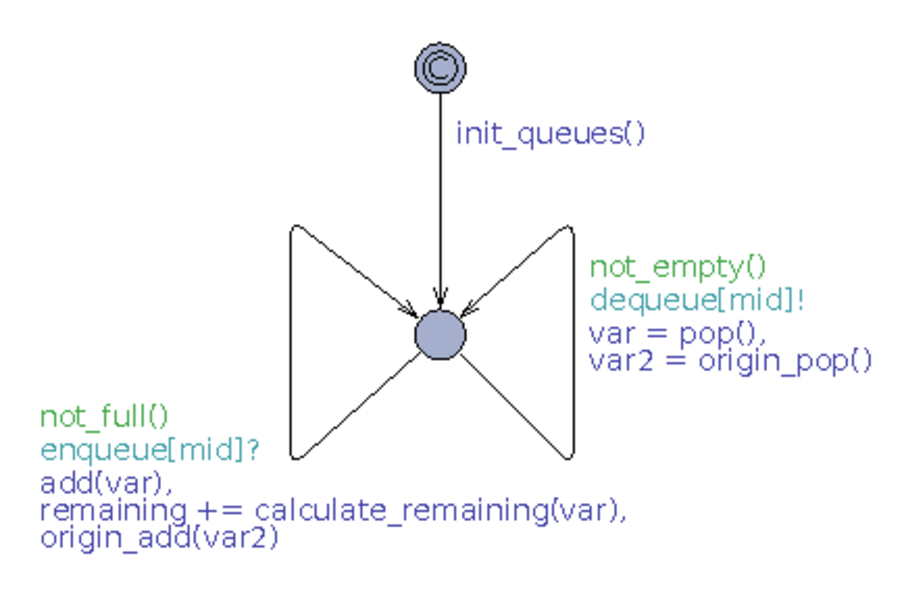
\includegraphics[width=\textwidth]{modulequeue.pdf}
\caption{The \textit{ModuleQueue} template}
\label{fig:modulequeue}
\end{figure}


\subsubsection{ModuleWorker Template}\label{subs:moduleworker}
The \emph{ModuleWorker} template can be seen in \cref{fig:moduleworker}. An instance of this template may apply several different types of work upon an item. In the \textit{Idle} location, the worker waits to synchronize with the module's \emph{ModuleQueue} instance allowing it to enter the \textit{Done} location. If the module can perform some work, it will move into the \emph{Working} location. Here it will wait for \emph{p\_time}, symbolizing the time it takes to perform the work. When the wait is over, it will try to synchronize with the item through the \emph{handshake} and \emph{work} channels as in the earlier version. Arriving at the \emph{Done} location, we may choose to work the item further if possible. Otherwise we perform a synchronization on the module's \emph{intern} channel. This passes the item over to the module's \emph{ModuleTransporter} instance. Synchronization on the intern channel may also occur, if the module can not perform any work on the item. This models the case, where an item has to pass through a module without having worked performed, while the model does not allow for pass through while it is working on other items.

\begin{figure}[H]
\centering
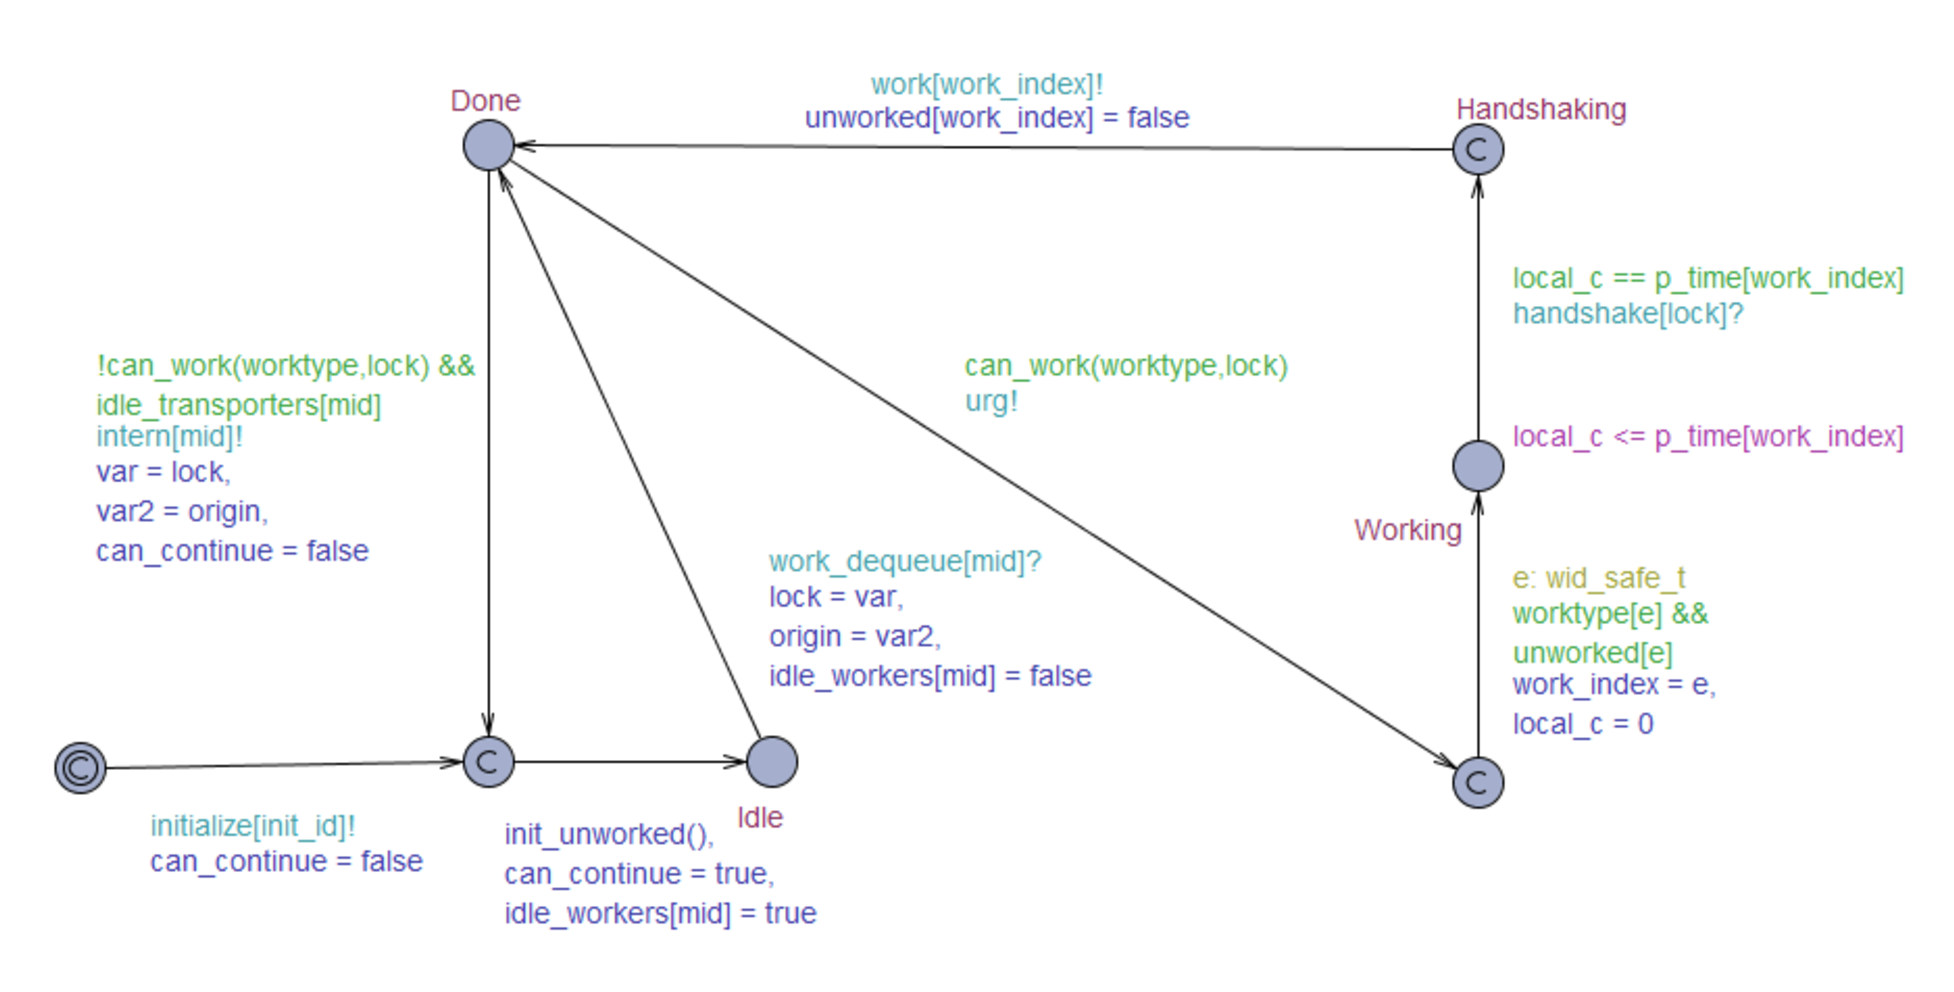
\includegraphics[width=\textwidth]{moduleworker.pdf}
\caption{The \textit{ModuleWorker} template}
\label{fig:moduleworker}
\end{figure}

\subsubsection{ModuleTransporter Template}
The \emph{ModuleTransporter} template can be seen in \cref{fig:moduletransporter}. A process of this template allows a module to transport an item onto a neighbouring module. If the item comes from the module's \emph{ModuleWorker} instance, then we move into the \emph{Selector} location by synchronizing on the module's \emph{intern} channel. We may however also move directly to the \emph{Selector} location by synchronizing with the module's \emph{ModuleQueue} instance over the \emph{dequeue} channel. This can however only be done, if the \cref{fig:moduletransporter} module allows us to pass an item through a module, while it is working on another item. This is indicated by the boolean \emph{pass\_through} variable, which is given at process instantiation. To create a module only used for transportation, we set this variable to \emph{true} and do not create a \emph{ModuleWorker} instance for the module. 

Once in the \emph{Selector} location a item may go to \emph{Idle} or \emph{Transporting}. If the item is done, it has to go back to \textit{Idle} and be removed from the production line by synchronizing on the \emph{remove} channel, as opposed to the \emph{transport[0]} in the earlier version. This also means that we do not specify a specific module to remove items from, they are just removed when done.

If the item is not done, it may look for a neighbouring module to be passed onto. A module may have up to four neighbours, one on each side. These are stored in the local \emph{next} array, their index indicating their placement relative to the module. When moving to \emph{Transporting} location, the item will choose a possible neighbour. In \emph{Transporting}, we wait to simulate the time taken to transport an item over the module. This time varies according to where the item enters the module, and where it leaves. The different transport times are stored in the 4 by 4 multidimensional \emph{t\_time} array. Given that we at this point know the direction, which the item entered from \emph{origin}, and the direction on which it will leave \emph{succ}, we can look up the exact time to wait in \emph{t\_time}. By implementing this feature, we ensure that the time take to pass over a module becomes more accurate to how an item may actually be transported over a module. 

Once the wait is over we move to the \emph{Queuing} location. If the neighbour's queue is full, we wait here until there is room. When possible we synchronize with the neighbours instance of \emph{ModuleQueue} using the \emph{enqueue} channel. At the same time we use the local \emph{inverse} function to calculate, from which side the item enters the neighbouring module. This is sent with the global \emph{var2} variable and is later saved into the  \emph{origin} variable of the neighbour's \textit{ModuleQueue} process. 

\begin{figure}[H]
\centering
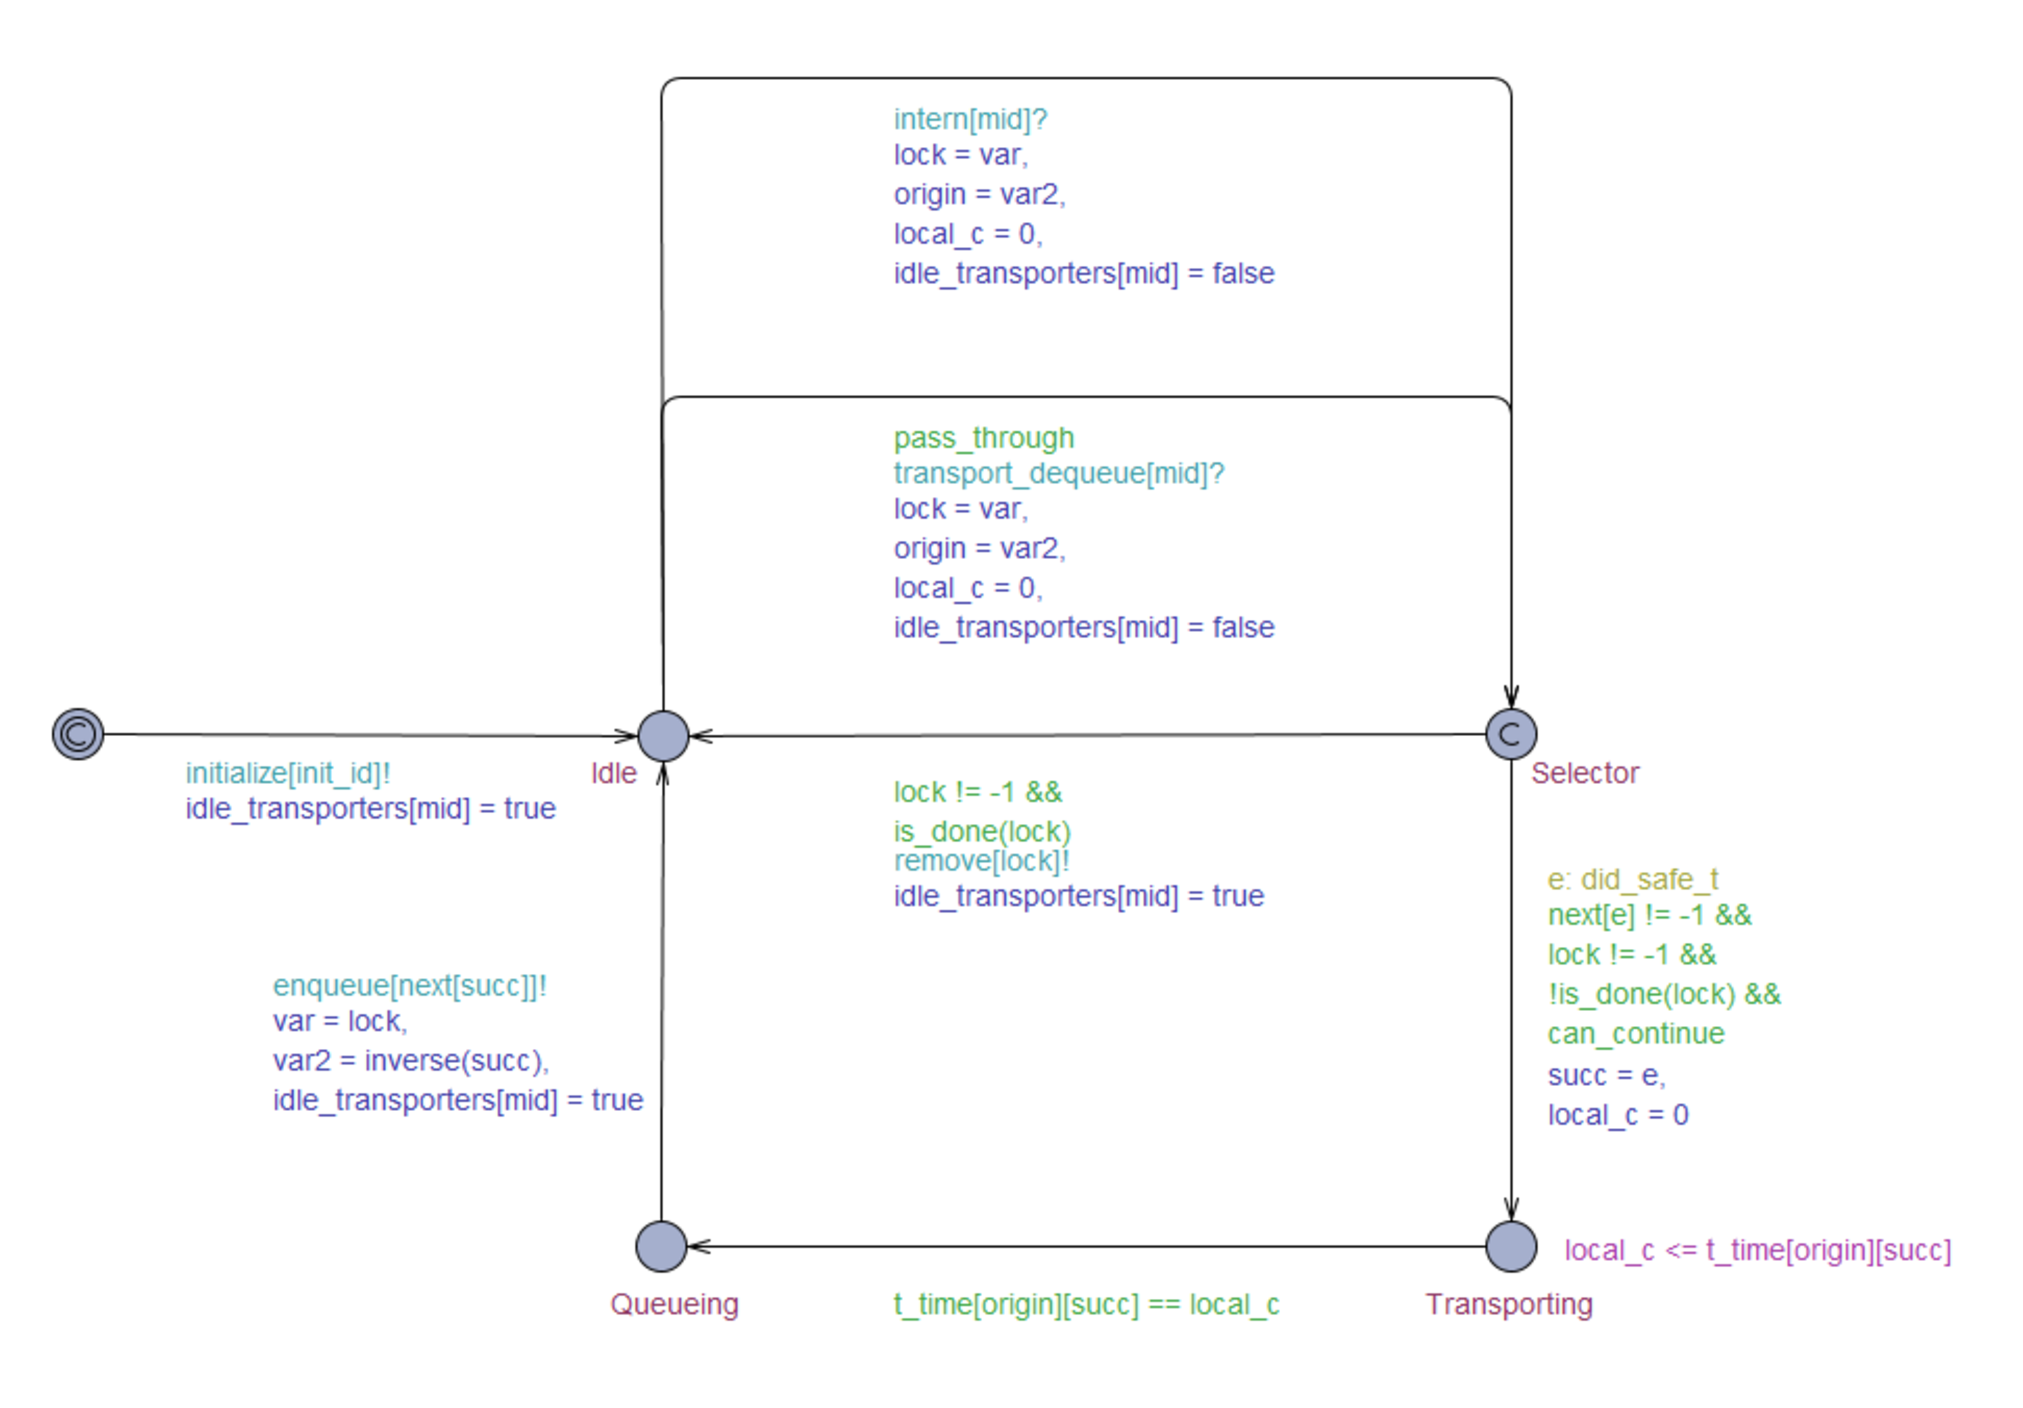
\includegraphics[width=\textwidth]{moduletransporter.pdf}
\caption{The \textit{ModuleTransporter} template}
\label{fig:moduletransporter}
\end{figure}



\section{Efficiency}\label{subs:efficiency}
\Cref{subs:recipequeue} illustrates how we make search for the shortest timed trace more efficient, by ordering how items are placed onto a factory. By applying such order, we are trying to keep down the global state space that needs to be searched, like how the bourgeois tries to keep down the proletariat. The lower the state space, the faster the search for the shortest timed trace.

This is not the only part of the model, where we combat the state space. We have strayed from going deeper into this until now, as it does not impact the overall functionality of the model. Yet it does greatly impact runtime. In the following subsections, we explain, how we have decreased our state space. 

\subsection{Urgencey}
The biggest positive impact on the state space has come through the use of committed locations and urgent channels. 

When a process enters a committed location, it ensures that globally no transition may be taken and no time may pass before the process leaves the location. This ensures that some processes stay atomic, such as handshake and work on item processes as described in \cref{subs:recipe}. This guards us from the interference of other processes, but also greatly reduces the state space, as we can not wait by making timed transitions in a commited location.

Urgency is an attribute that can be applied to different channels. Having a channel be urgent means that no time may pass, if we can transition from one process to another by synchronizing on the channel. In \emph{ModuleWorker} on \cref{subs:moduleworker} the \textit{Intern} channel is urgent. This means that, when the guards evaluate to true, then we transition by synchronizing on \emph{intern}. Again, not allowing the system the possibility of waiting reduces the state space.

There are transitions going between locations that we wish to make urgent, such as from \emph{Done} to \emph{Working} in the \textit{ModuleWorker} template, where there is not already some way of synchronizing on a channel. We solve this by creating a new simple template called \emph{Urgent}. A process instantiated from this will continuously try to synchronize on the urgent \emph{urg} channel. Thus we can add a synchronization on this channel to any non-urgent transition to make it urgent. 

A big difficulty with working with committed locations and urgent channels is that we sometimes need to be able to wait. This is the case when passing from \emph{ModuleWorker} to \emph{ModuleTransporter} through the intern channel as mentioned above. We can not safely make \emph{intern} urgent, if we may synchronize on it from \emph{ModuleWorker} but not \emph{ModuleTransporter}. This will lead to unwanted deadlock. Therefore, the guard on this particular transition states that it must only be taken, if the \emph{ModuleTransporter} is in idle and can communicate. We use this technique throughout the model, applying guards so that we may safely make our channels urgent. 

\subsection{Priority}
In order to shave more off the state space, we have also create priorities between channels using the built-in UPPAAL priority feature. This can be seen in \cref{code:cp}. By placing this order, we do not allow the model checker to synchronize on a certain channel, if a channel of a higher priority may be synchronized on. This helps guide us when there is an ambiguous choice of which channel to communicate on.

However, if we set up the same configuration in a version of the UPPAAL model without priorities and one with, then their initial parallel processes will not be bisimilar. This is because the model with priorities is restricted from transitions that the un-priotitized model may take. Yet, we find that this does not impact the fastest schedule found between the two different set ups. By design of the templates, none of the processes that make up the larger parallel system process will be able to make another transition, if they are waiting to communicate on a channel. Because of this, if two processes waiting to communicate are bypassed because of prioritization, they will stick around and wait. Resulting from the nature of the system, they will be able to communicate before the global clock is counted up, which only occurs as the result of transport and work on items. Because of this, our shortest time schedules end up having their final global clock values be equal, whether we prioritize or not.  

An issue is that even with channel priorities, we may have two transitions communicating on the same channel type, which again leaves us with an ambiguous order of execution. To get around this, we also prioritize system instances. If we ever get into the above situation, we pick the transition involving instances with the highest priorities. 

\lstinputlisting[language=C, caption=Channel priorities, captionpos = b, label={code:cp}, float]{codeRelated/UPPAAL/channelpriorities.txt}

\subsection{Initial Order}
A feature which UPPAAL templates lack is a user-defined constructor, which would allow us to execute code right when a process is made. We need this feature in templates such as \emph{ModuleQueue} in \cref{subs:modulequeue}, where we need to set up an array implementing the local queue. To get around this, we add an initial location to the template. To transition from this location, the instantiating functions have to be called.

The issue here is that with N processes having to be instantiated in this manner, there are N! ways of performing instantiation. This greatly increases our state space. To get around this, we use a queueing system similar to \emph{RecipeQueue} in \cref{subs:recipequeue}. This is implemented with the \emph{Initializer} template as seen in \cref{fig:initializer}. Each process, which needs to have code run upon instantiation, is given an instantiation id. When creating a procsses from the \emph{Initializer} template, we give it an array, which orders all these ids. The \emph{Initializer} process then starts to instantiate the instances in the order given to it by synchronizing on the \emph{initialize} channel. As the \emph{Initializer} process's main location is committed, nothing may occur until all needed instances have been synchronized with. Once all instantiations have been done, the \emph{Intanializer} is forced to move into a dead state, and we need not to worry about it anymore. From this point on the remaining  processes can transition as before. 

\begin{figure}[h]
\centering
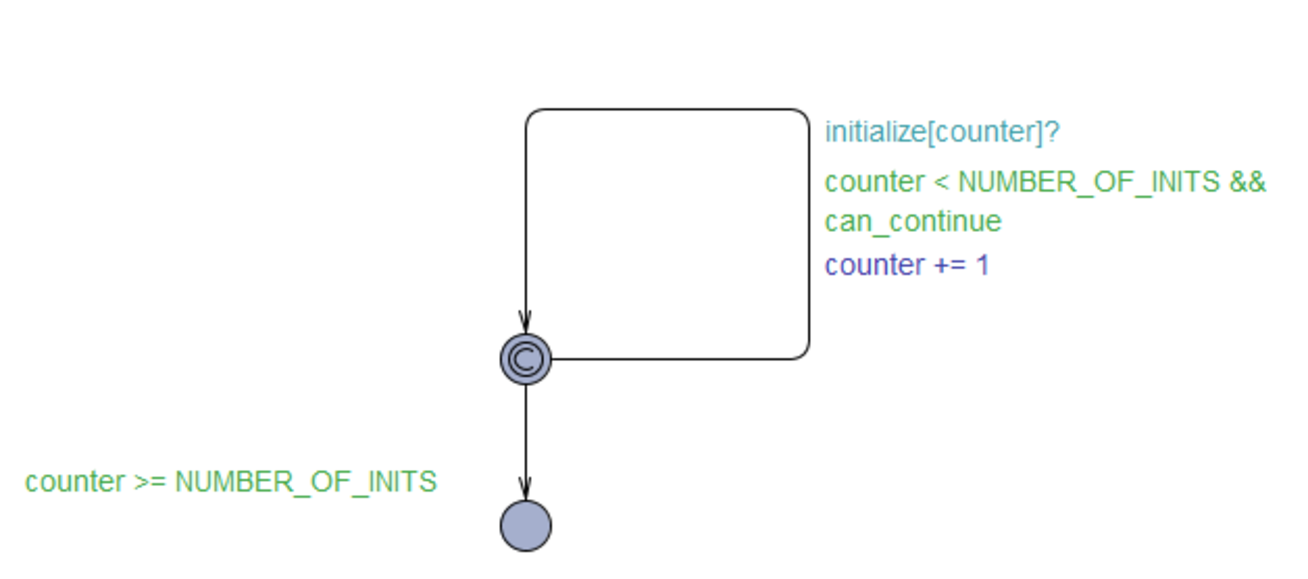
\includegraphics[width=\textwidth]{init.pdf}
\caption{The \textit{Initialzier} template}
\label{fig:initializer}
\end{figure}


\section{Evaluation of Model}
Having now defined all needed templates as to model a factory configuration in UPPAAL, we would like to evaluate our design. We will evaluate, how well our model is capable of emulating reality. This is done by comparing the time it takes for a real life factory configuration to produce an order items, to the rating we give the same configuration when simulated in UPPAAL. 

\subsection{The Model Compared to Reality} \label{ssec:realcomparison}
In order to compare our model to reality, we set up the configuration of the actual CP Learning Factory mentioned earlier using our UPPAAL templates. We then run different orders on both the actual factory and the model. Afterwards, we compare the time it takes for both to produce their orders.  

The configuration, which we wish to simulate, is used to produce faux smartphones. 3 different recipes were set up, which described different types of smartphones that the configuration may produce. These can be seen in \cref{fig:cp-recipes}. Each are named after, how many fuses are put into them.

\begin{figure}[h]
\centering
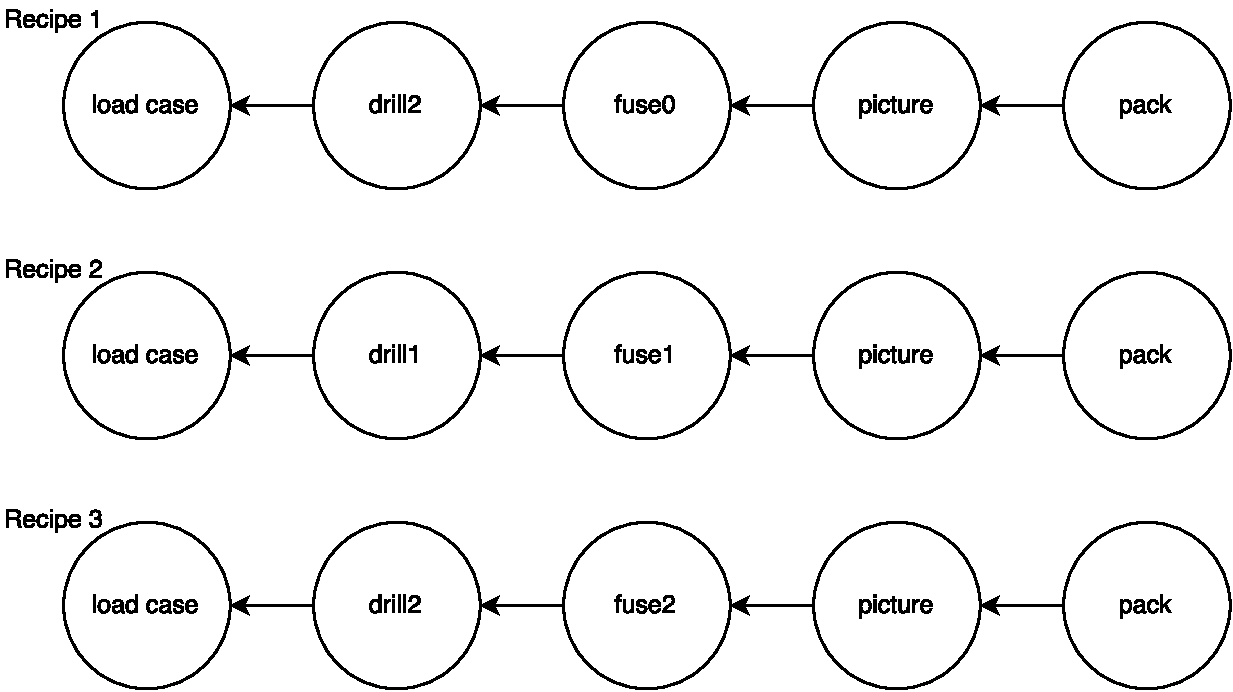
\includegraphics[width=0.5\textwidth]{cp-recipes.pdf}
\caption{Dependency graphs representing the three recipes the CP-Factory could produce}
\label{fig:cp-recipes}
\end{figure}

Inspecting the configuration, we find the different modules and the types of work that they may perform, as well as how they connect. This is shown in \cref{fig:cp-setup}. We choose to disregard that these modules each have two conveyor belts, as both are not used by any item produced. We also disregard the \textit{Transport1} module, as it is not used in the production of any item.

\begin{figure}[h]
\centering
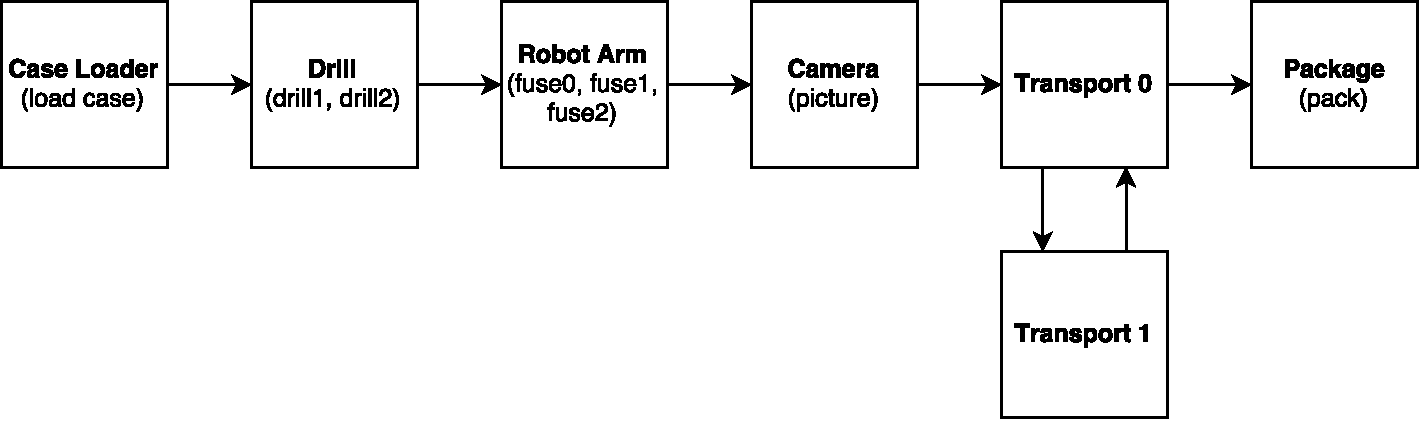
\includegraphics[width=\textwidth]{cp-setup.pdf}
\caption{Graphical representation of the CP-Factory configuration at Aalborg University}
\label{fig:cp-setup}
\end{figure}

Each item is placed on the configuration in the \textit{Case Loader} module and are removed at the \textit{Package} module. We were allowed to try and produce some items using the factory. Here we timed how long it takes for items to pass over modules, and how long it takes for certain works to be done. Averages of these times are listed in \cref{tab:cp-time}.

\begin{table}[]
\centering
\begin{tabular}{ccccc}
\multicolumn{1}{l}{} & \multicolumn{1}{l}{PLACE HOLDER} & \multicolumn{1}{l}{TABLE} & \multicolumn{1}{l}{PLACE} & \multicolumn{1}{l}{HOLDER} \\
recipe 1             & 69                               & 69                        & 69                        & 69                         \\
recipe 2             & 69                               & 69                        & 69                        & 69                         \\
recipe 3             & 69                               & 69                        & 69                        & 69                        
\end{tabular}
\caption{Table showing the time it took for transport through and do different kinds of work on modules. Times are in milliseconds}
\label{tab:cp-time}
\end{table}

In total we ran four different orders on the configuration. On \cref{tab:orders} each order is defined by the item types it needs to produce, as well as the amount of each type required.   

\begin{table}[htb]
\centering
\begin{tabular}{|l|l|}
\hline
{\ul \textbf{Order Name}} & {\ul \textbf{Description}}                                                    \\ \hline
\textbf{SingleNoFuse}     & NoFuse: 1                                                                     \\ \hline
\textbf{SingleLeftFuse}   & LeftFuse: 1                                                                   \\ \hline
\textbf{SingleBothFuse}   & BothFuse: 1                                                                   \\ \hline
\textbf{AllTypes}         & \begin{tabular}[c]{@{}l@{}}NoFuse: 1\\ LeftFuse: 1\\ BothFuse: 1\end{tabular} \\ \hline
\end{tabular}
\caption{Describes each order by the item types to produce as well as the amount of each.}
\label{tab:orders}
\end{table}


With all this in place, we are able to set up the configuration in UPPAAL using our templates and running each of the four orders on it. In \cref{app:festoex} is shown how we set up the system to run the \textit{AllTypes} order. Please note that the \textit{Item} template is here called \textit{Recipe} and similarly \textit{ItemQueue} is called \textit{RecipeQueue}. The variables \textit{recipe0}, \textit{recipe1} and \textit{recipe2} refer to the 3 processes, which represent the three items that need to be produced for the \textit{AllTypes} order. At the bottom of the example, we see how we parallelize all the smaller processes into one big system process. For this case the following reachability query is given to the UPPAAL model checker:
\\ \\
$E<>\textit{ }recip0.done\textit{ and }recipe1.done\textit{ and }recipe2.done$
\\ \\
It asks: \textit{"From the initial state, can we reach a state where all three items have been completed"}. A similar query is used for the three simpler orders. In all cases it evaluates to true. Because of this we can produce the shortest timed trace for each order, and on the last state read the value of the global clock. This is the configuration's rating given the specific order, which describes how long it takes to run the fastest schedule. Having extracted this from each of the four orders, we compare them with the time it takes to complete the orders on the actual factory configuration. The results of this can be seen in \cref{tab:cp-results}.

\begin{table}[htb]
\centering
\begin{tabular}{|l|l|l|l|}
\hline
{\ul \textbf{Order Name}} & {\ul \textbf{Actual}} & {\ul \textbf{Simulated}} & {\ul \textbf{Difference}} \\ \hline
\textbf{SingleNoFuse}     & 144.8                 & 144.9                    & 0.1                       \\ \hline
\textbf{SingleLeftFuse}   & 156.5                 & 156.6                    & 0.1                       \\ \hline
\textbf{SingleBothFuse}   & 171.6                 & 171.7                    & 0.1                       \\ \hline
\textbf{AllTypes}         & 305                   & 311                      & 6                         \\ \hline
\end{tabular}
    \caption{Comparison of actual and simulated times. Time is in milliseconds.}
    \label{tab:cp-results}
\end{table}

Looking at the results, we are almost spot on for the very simple orders. Yet the simulated and actual time drift a bit apart as the orders becomes more complex, though still to a small degree in our case. These results will be discussed further in \cref{sec:modeling}.
